\cotefile{156-7}
\scanpage{2}
\mspage{1}
\margin{\tikz[baseline=(h.base)]{\node[inner sep=2pt] (h) {\unsure{GF|CF} VII}; \draw (h.north west)--(h.south west)--(h.south east);}}
\begin{center}Analysis Situs (troisième mouture)\end{center}
% slanted
\margin{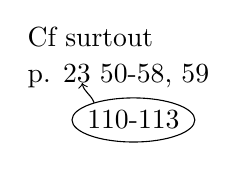
\begin{tikzpicture}[baseline=(n.base),x=1cm,y=1cm]
\node[anchor=west,inner sep=0pt] (n) at (0,0) {Cf surtout};
\node[anchor=west,inner sep=0pt] at (0,-0.5) {p. 23 \unsure{50}-58, 59};
\node[inner sep=1pt] (r) at (1.35,-1.05) {110-113};
\draw (1.35,-1.05) ellipse (0.78 and 0.28);
\draw[->] (0.85,-0.83) to[out=110,in=-80] (0.70,-0.58);
\end{tikzpicture}}

\uline{23 juin}

Je récapitule les données et axiomes d'une ``algèbre des figures'', ou ``\uline{atelier}''. Il s'agit pour l'instant d'axiomes purement ``algébriques'' dominant le formalisme algébrique des figures, à l'exclusion pour le moment des propriétés topologiques (densité, connexité, acyclicité) ou \inserted{\uline{proprement}} géométriques (régularité topologique, boules et sphères topologiques d'une algèbre de figures), voire les ``propriété combinatoires fines'', autour de la notion de \unsure{simplexe|simplexes}.

Parmi les axiomes, je distingue les axiomes ``sine qua non'' At~1 à At~7, qui me paraissent les plus essentielles pour fonder le sens géométrico-topologique du formalisme envisagé. Les autres axiomes seront considérés comme plus ou moins ``\unsure{facultatif|facultatifs}'' au niveau du formalisme algébrique. Ils pourront sans doute un rôle crucial, dès qu'il s'agira d'un travail sur pièces dans le
